\documentclass[10pt]{scrartcl}

\usepackage[utf8]{inputenc}
\usepackage{tabularx}
\usepackage{longtable}
\usepackage[ngerman]{babel}
\usepackage[automark]{scrpage2}
\usepackage{amsmath,amssymb,amstext}
\usepackage[]{color}
\usepackage[]{enumerate}
\usepackage{graphicx}
\usepackage{polynom}
\usepackage{lastpage}
\usepackage[perpage,para,symbol*]{footmisc}
\usepackage{listings} 
\usepackage[pdfborder={0 0 0},colorlinks=false]{hyperref}
\usepackage[numbers,square]{natbib}
\usepackage{color}
\usepackage{colortbl}
\usepackage[absolute]{textpos}
\usepackage{float}
\usepackage[colorinlistoftodos,textsize=small,textwidth=2cm,shadow,bordercolor=black,backgroundcolor={red!100!green!33},linecolor=black]{todonotes}

\lstset{numbers=left, numberstyle=\tiny, numbersep=5pt, breaklines=true, showstringspaces=false} 
\restylefloat{figure}

%changehere
\def\titletext{Uebungsblatt 2}
\def\titletextshort{Uebungsblatt 2}
\author{André Harms, Oliver Steenbuck}

\title{\titletext}

%changehere Datum der Übung
\date{24.05.2012}

\pagestyle{scrheadings}
%changehere
\ihead{TH1, Padberg}
\ifoot{Generiert am:\\ \today}

\cfoot{Oliver Steenbuck, André Harms}


\ohead[]{\titletextshort}
\ofoot[]{{\thepage} / \pageref{LastPage}}

\setlength{\parindent}{0.0in}
\setlength{\parskip}{0.1in}

\begin{document}
\maketitle

\setcounter{tocdepth}{3}
\tableofcontents

%	\listoftables                                 												% 
	\listoffigures  
%	\lstlistoflistings	

\section{Aufgabe 1}
	\subsection{Aufgabe 1.1}
			\begin{figure}[H]
    			\centering
				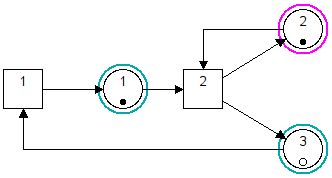
\includegraphics[scale=0.5]{aufg1.png}		
            	\caption{Aufgabe 1 Petri Netz}
            	\label{petri:aufg1}
			\end{figure}


			\begin{figure}[H]
    			\centering
				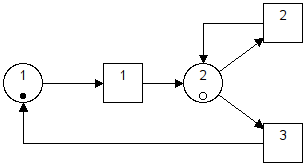
\includegraphics[scale=0.5]{aufg1Dual.png}		
            	\caption{Aufgabe 1 Petri Netz Dual}
            	\label{petri:aufg1:dual}
			\end{figure}
			
	\subsection{Aufgabe 1.2}
		\subsubsection{N}
		
		pre =
		$\begin{pmatrix} N/A & T1 & T2 \\
						 S1 & 0 & 1 \\
						 S2 & 0 & 1 \\
						 S3 & 1 & 0 \end{pmatrix}$ \\ 
						 
		post =
		$\begin{pmatrix} N/A & T1 & T2 \\
						 S1 & 1 & 0 \\
						 S2 & 0 & 1 \\
						 S3 & 0 & 1 \end{pmatrix}$ \\ 
						 
		Inzidenzmatrix = $post - pre$ = $\begin{pmatrix} N/A & T1 & T2 \\
						 S1 & 0 & 1 \\
						 S2 & 0 & 1 \\
						 S3 & 1 & 0 \end{pmatrix}  - \begin{pmatrix} N/A & T1 & T2 \\
						 S1 & 1 & 0 \\
						 S2 & 0 & 1 \\
						 S3 & 0 & 1 \end{pmatrix}$  = $\begin{pmatrix} 
						 -1 & 1 \\
						 0 & 0 \\
						 1 & -1 \end{pmatrix}$\\
		S-Invarianten = ($I^T \cdotp I_p = \overrightarrow{0}) = \begin{pmatrix} 
						 -1 & 0 & 1 \\
						 1 & 0 & -1\end{pmatrix} \cdotp I_p= \overrightarrow{0}$ \\
		Lösung und damit S Invarianten = $k_1 \cdotp \begin{pmatrix} 
						 1 \\
						 0 \\
						 1 \end{pmatrix}$, $k_2 \cdotp \begin{pmatrix} 
						 0 \\
						 1 \\
						 0 \end{pmatrix}$\\

		T-Invarianten = $(I \cdotp I_t) = \overrightarrow{0} = \begin{pmatrix} 
						 -1 & 1 \\
						 0 & 0 \\
						 1 & -1 \end{pmatrix} \cdotp I_p = \overrightarrow{0}$\\
		
		Lösung und damit T Invarianten = $\begin{pmatrix} 
						 1 \\
						 1\end{pmatrix}$\\

	
		\subsubsection{Dual(N)}
		
		pre =
		$\begin{pmatrix} N/A & T1 & T2 & T3\\
						 S1 & 1 & 0 & 0 \\
						 S2 & 0 & 1 & 1\end{pmatrix}$  
						 
		post =
		$\begin{pmatrix} N/A & T1 & T2 & T3\\
						 S1 & 0 & 0 & 1 \\
						 S2 & 1 & 1 & 0\end{pmatrix}$ 
						 
						 
		Inzidenzmatrix = $post - pre$ = $\begin{pmatrix} N/A & T1 & T2 & T3\\
						 S1 & 0 & 0 & 1 \\
						 S2 & 1 & 1 & 0\end{pmatrix}  - \begin{pmatrix} N/A & T1 & T2 & T3\\
						 S1 & 1 & 0 & 0 \\
						 S2 & 0 & 1 & 1\end{pmatrix}$  = $\begin{pmatrix} 
						 -1 & 0 & 1 \\
						 1 & 0 & -1 \end{pmatrix}$
		\\S-Invarianten = $(I^T \cdotp I_p) = \overrightarrow{0} = \begin{pmatrix} 
						 -1 & 1\\
						 0 & 0\\
						 1 & -1 \end{pmatrix} \cdotp I_p = \overrightarrow{0}$\\ 
		Lösung und damit S Invarianten = $\begin{pmatrix} 
						 1 \\
						 1\end{pmatrix}$\\
						 
		T-Invarianten = $(I \cdotp I_t) = \overrightarrow{0} = \begin{pmatrix} 
						 -1 & 0 & 1 \\
						 1 & 0 & -1 \end{pmatrix} \cdotp I_p = \overrightarrow{0}$\\
		
		Lösung und damit T Invarianten = $k_1 \cdotp \begin{pmatrix} 
						 1 \\
						 0 \\
						 1 \end{pmatrix}$, $k_2 \cdotp \begin{pmatrix} 
						 0 \\
						 1 \\
						 0 \end{pmatrix}$\\
						 
	\subsubsection{Aufgabe 1.3}
	Durch das Transponieren der Inzidenzmatrix in der Funktion $D(N)$ kann $I_D$ auch ausgedrückt werden als $I_N^T$ wodurch $I_D \cdot I_{Dt} = I_N^T \cdot I_{Np} = \overrightarrow{0}$
	
\section{Aufgabe 2}
\begin{enumerate}

	\item \textbf{korrekt} - Reversibel heißt es kann von jedem Knoten jeder andere Knoten durch eine Reihe von Transitionen erreicht werden. Der Kondensationsgraph enthält für jede menge $D_i$ von Knoten einen Knoten wenn die Knoten in $D_i$ stark d.h. in beide Richtungen miteinander verbunden sind. Wenn der Kondensationsgraph mehr als einen Knoten enthält kann die Transition zwischen diesen Knoten nicht in beide Richtungen durchlaufen werden. Das Netz ist an dieser stelle also nicht reversibel.
	
	
	\item 	\begin{figure}[H]
    			\centering
				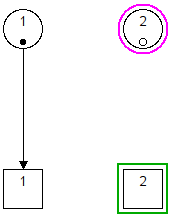
\includegraphics[scale=0.5]{aufg2.png}		
            	\caption{Aufgabe 2.2 Petri Netz}
            	\label{petri:aufg22}
			\end{figure}
	Das in Abbildung \ref{petri:aufg22} gezeigte Netz hat als S und T Invarianten $\begin{pmatrix} 
						 0 \\
						 1 \end{pmatrix}$ ist aber nicht reversibel wenn $T_1$ geschaltet wird. Damit gilt die Aussage nicht für alle Netze.
						 
						 
	\item Nein beispielsweise der EG und der KG für das in Abbildung \ref{petri:aufg23} gezeigte Netz.
	
	\begin{figure}[H]
    			\centering
				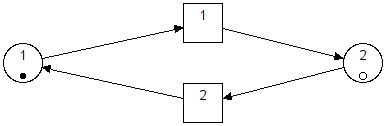
\includegraphics[scale=0.5]{aufg23.png}		
            	\caption{Aufgabe 2.3 Petri Netz}
            	\label{petri:aufg23}
			\end{figure}	
	
	\item Korrekt, weil dann alle Transitionen einmal geschaltet werden.
	
	\item Inkorrekt, gegeben eine Transaktion die auf einen Knoten zwei Token auflegt und eine andere die von diesem Knoten immer wieder zwei herrunternimmt ist der EG unendlich und der KG besteht nur aus einem Knoten.
	
	
\end{enumerate}
\section{Aufgabe 3}
Das Netz ist nicht Deadlockfrei. Die Schaltreihenfolge $t2 \rightarrow t3 \rightarrow t2$ führt zu einem Deadlock. Siehe auch Abbildung \ref{petri:aufg3}
	\begin{figure}[H]
    			\centering
				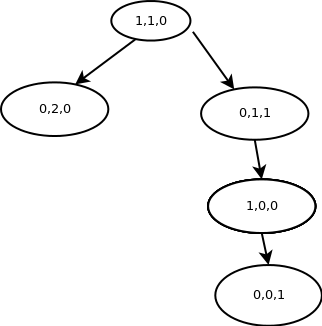
\includegraphics[scale=0.5]{aufg3.png}		
            	\caption{Aufgabe 3 UG}
            	\label{petri:aufg3}
			\end{figure}

\section{Aufgabe 4}
	\begin{figure}[H]
    			\centering
				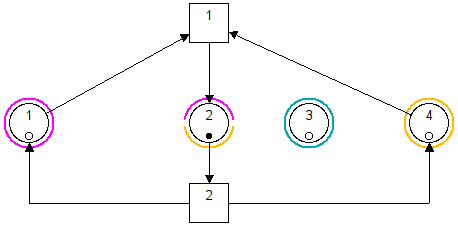
\includegraphics[scale=0.5]{aufg4.png}		
            	\caption{Aufgabe 4 Petri Netz}
            	\label{petri:aufg4}
			\end{figure}
	\begin{align*}
		pre = \begin{pmatrix} N/A & T1 & T2 \\
						 S1 & 1 & 0 \\
						 S2 & 0 & 1 \\
						 S3 & 0 & 0 \\
						 S4 & 1 & 0 \end{pmatrix}\\ 	
		post = \begin{pmatrix} N/A & T1 & T2 \\
						 S1 & 0 & 1 \\
						 S2 & 1 & 0 \\
						 S3 & 0 & 0 \\
						 S4 & 0 & 1 \end{pmatrix}\\
		invarianz = \begin{pmatrix}
						 -1 & 1 \\
						 1 & -1 \\
						 0 & 0 \\
						 -1 & 1 \end{pmatrix}\\
		\textit{S-Invarianten} = (I^T \cdotp I_p = \overrightarrow{0}) = \begin{pmatrix}
						 -1 & 1 & 0 & -1\\
						 1 & -1 &0 & 1\end{pmatrix}
		\cdot I_p = \overrightarrow{0}\\ 
		\textit{Durch scharfes hinsehen ergibt sich die relevante Lösung und damit S Invariante} = \begin{pmatrix} 
						 1 \\
						 2\\
						 0\\
						 1\end{pmatrix}				 		 				  				 			
	\end{align*}


\end{document}
